\section{Relativistic Energy Conservation}
%By Matt Trawick.

\makelabheader %(Space for student name, etc., defined in master.tex)

\bigskip
\vspace{\fill}

\textbf{Introduction}

The \textit{classical} expression\footnote{Physicists use the term \textit{classical} to refer to physics as it was before the twin revolutions of relativity and quantum mechanics, both of which 
took place in the early 1900s.  Thus ``classical mechanics'' refers to nonrelativistic motion of macroscopic objects as it was understood before Einstein's special relativity in 1905, and ``classical electrodynamics'' refers to electromagnetic fields and waves as they were understood before the modern conception of the of the photon---also due to Einstein and also in 1905, in what physicists refer to as ``having a good year.''
}
for kinetic energy, $K=\frac{1}{2}mv^2$, is incorrect at high speeds, because it implies that an object traveling at just under the speed of light could  increase its kinetic energy by just a little bit and end up with a speed \textit{above} the speed of light---which is impossible.  The correct expression for kinetic energy is
\begin{equation}
K=(\gamma -1)mc^2.
\label{eq:K_relativistic}
\end{equation}
This new expression looks weird at first because it doesn't seem to depend on velocity at all, but in fact the velocity dependence is hidden inside $\gamma$.  We can be expand it to show the velocity dependence explicitly as 
\begin{equation}
K=\left[ \left(1 - \frac{u^2}{c^2} \right)^{-\frac{1}{2}} - 1 \right]mc^2,
\end{equation}
following our usual convention of denoting velocities by $u$ for objects and $v$ reference frames. 
In this lab, you will
% analyze several example collisions to 
explore how this new, relativistic expression for $K$ changes our understanding of the conservation of energy.

\bigskip

\textbf{Activity 1: Kinetic Energy in a Collision}

Bob watches as two objects (or \textit{particles}), with equal mass $m$, collide and stick together.  In Bob's reference frame, the two particles initially have the same speed $u=0.6c$ but in opposite directions; the resulting larger particle has speed $u_{\rm f}=0$.

\begin{figure}[h!]
\begin{center}
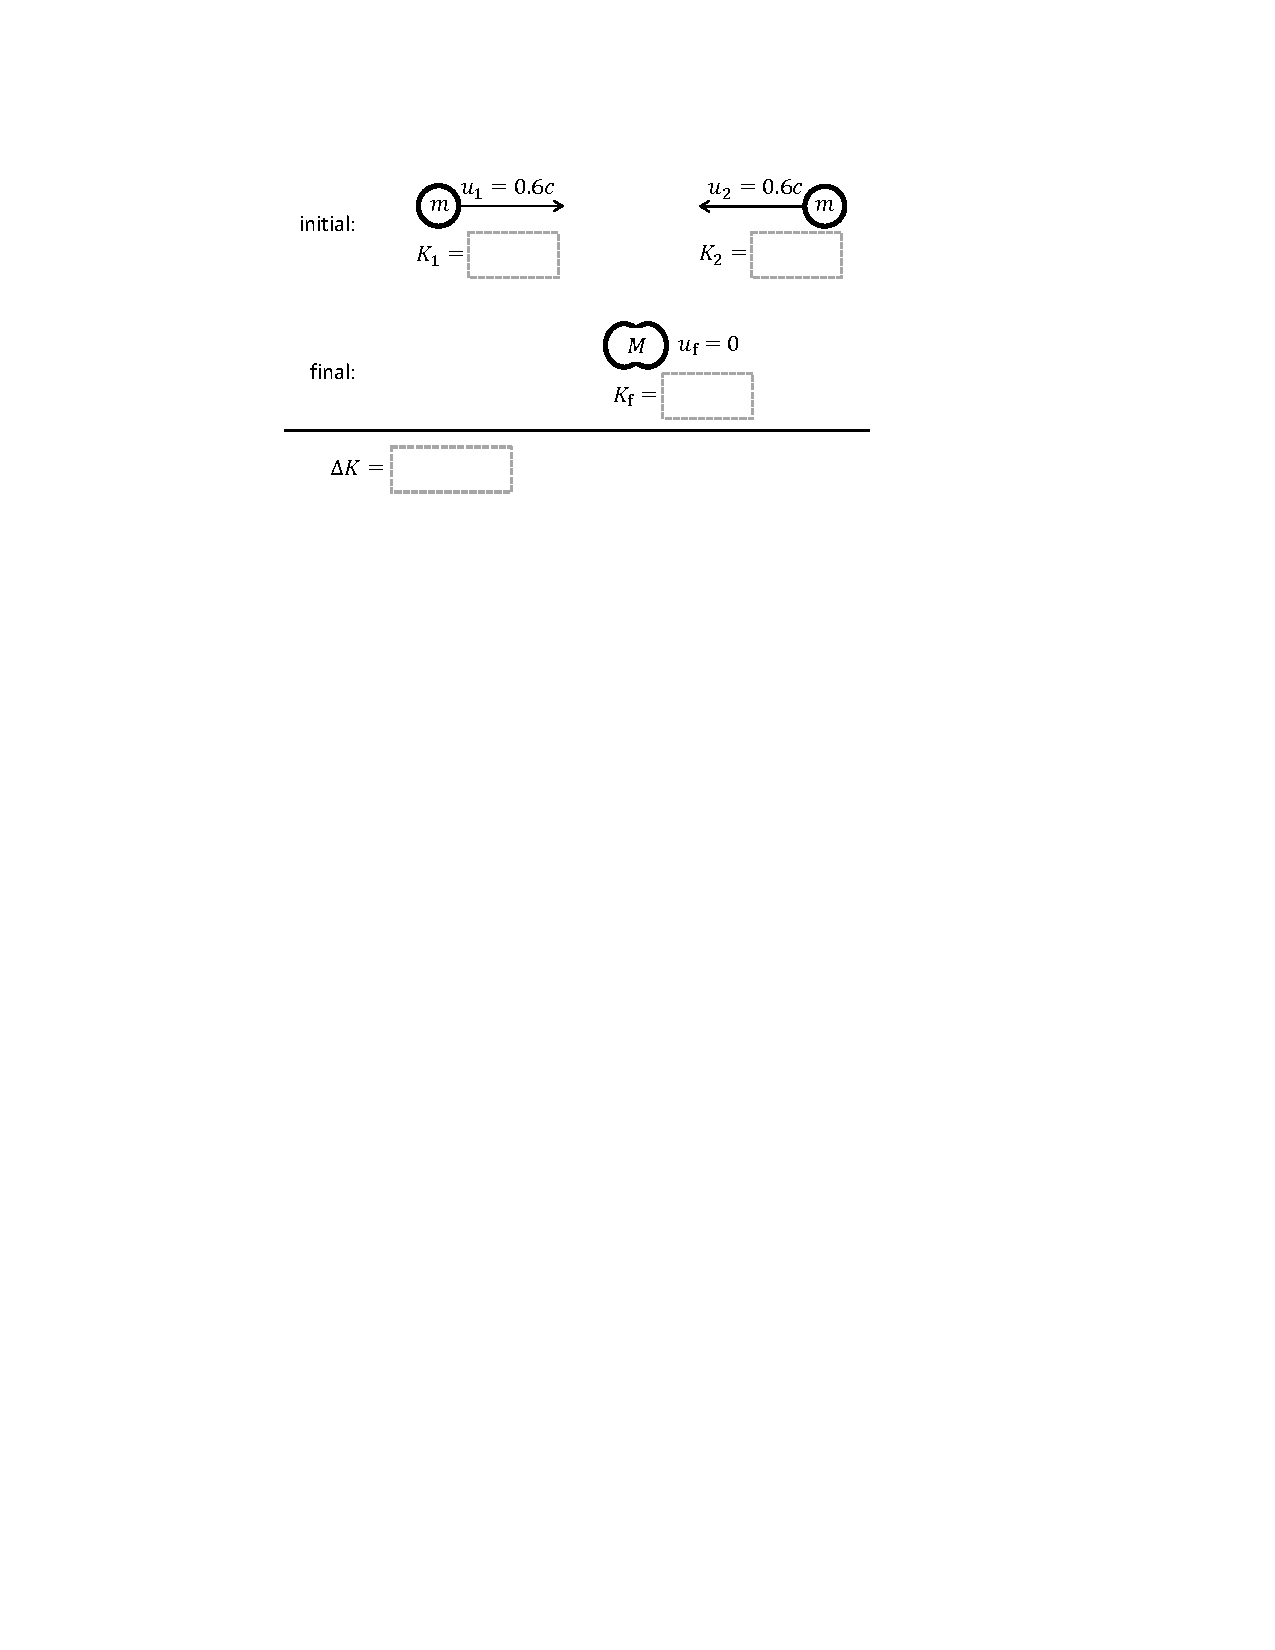
\includegraphics{energy_mass/collision_m_and_m.pdf}
\caption{Bob's reference frame.}
\label{figure_collision_m_and_m_bob}
\end{center}
\end{figure}

\begin{enumerate}[labparts]
\item Use Equation~1 above to calculate the kinetic energy $K$ of each particle in the figure above.  Since you're not given any numbers for the masses, it's fine to write all of your final answers as multiples of ``$mc^2$''.
\answerspace{0.3in}

\item Calculate the change in the kinetic energy $\Delta K = K_{\rm final} - K_{\rm initial}$, being careful with your signs.  
\answerspace{0.3in}

\pagebreak

Anna also observes the collision between the two particles, but she does so while speeding by Bob at $+0.6c$, the same velocity as the first particle.  In Anna's reference frame, $v=+0.6c$, the first particle has $u'_1=0$.

\begin{figure}[h!]
\begin{center}
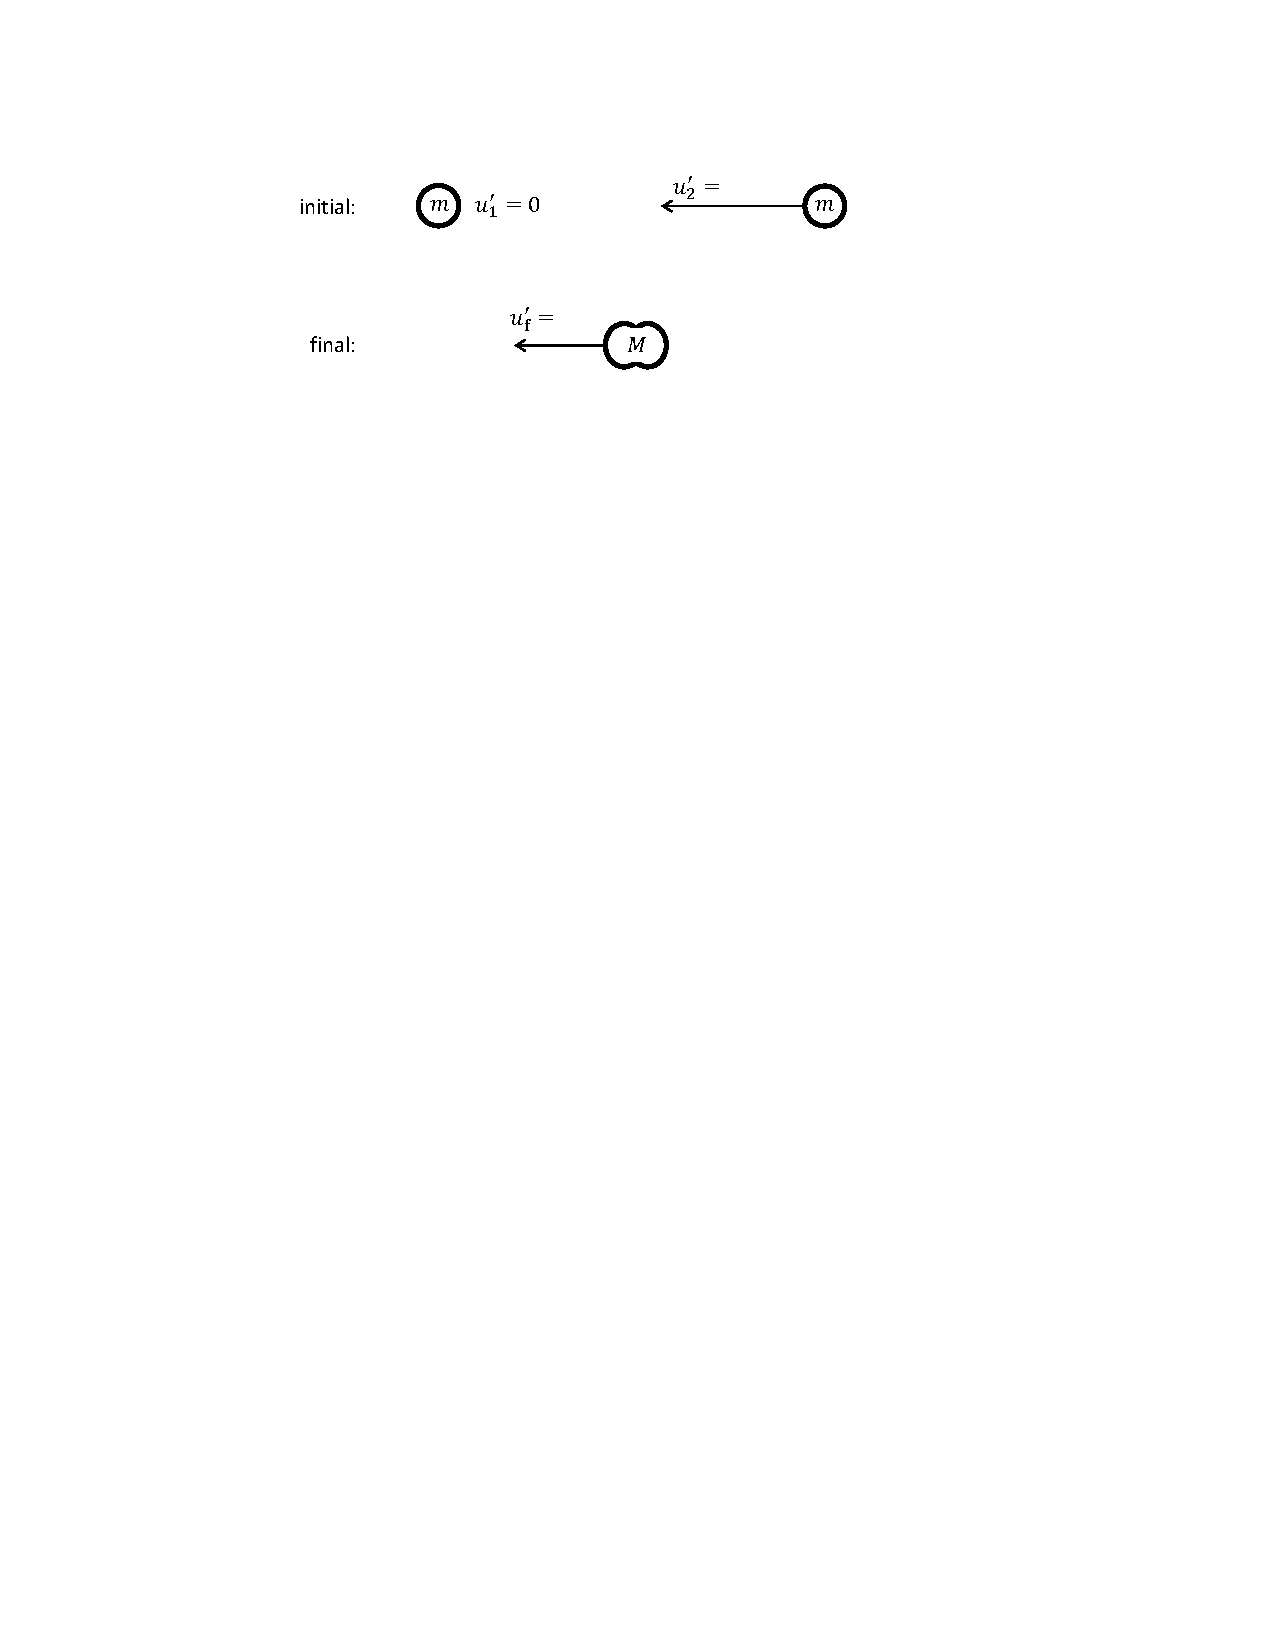
\includegraphics{energy_mass/collision_m_and_m_anna_no_k.pdf}
\caption{Anna's reference frame.}
\label{figure_collision_m_and_m_anna_no_k}
\end{center}
\end{figure}

\item Calculate the speeds $u'_2$ and $u'_{\rm f}$ of the other particles in Anna's reference frame in the figure above.
\answerspace{0.8in}

\end{enumerate}

\textbf{Activity 2: What Do Anna and Bob Agree On?}

Let's consider what Anna and Bob do and don't agree on based on their reference frames.  Of course, they disagree about the velocities of individual particles, as $u' \neq u$ in all cases.  And since they disagree on the particles' velocities, they surely disagree on their kinetic energies $K$ as well.  But what about the overall change in kinetic energy $\Delta K$ during the collision?  Should they agree on that?

To address this question, we'll imagine a specific latching mechanism that causes the two objects to remain together after they collide.  In the figure below, each object includes a spring that gets compressed during the collision, with some of the initial kinetic energy of the two particles going towards compressing the springs.  If the springs don't get compressed enough, the latch won't close, and the particles won't stay together.

\begin{figure}[h!]
\begin{center}
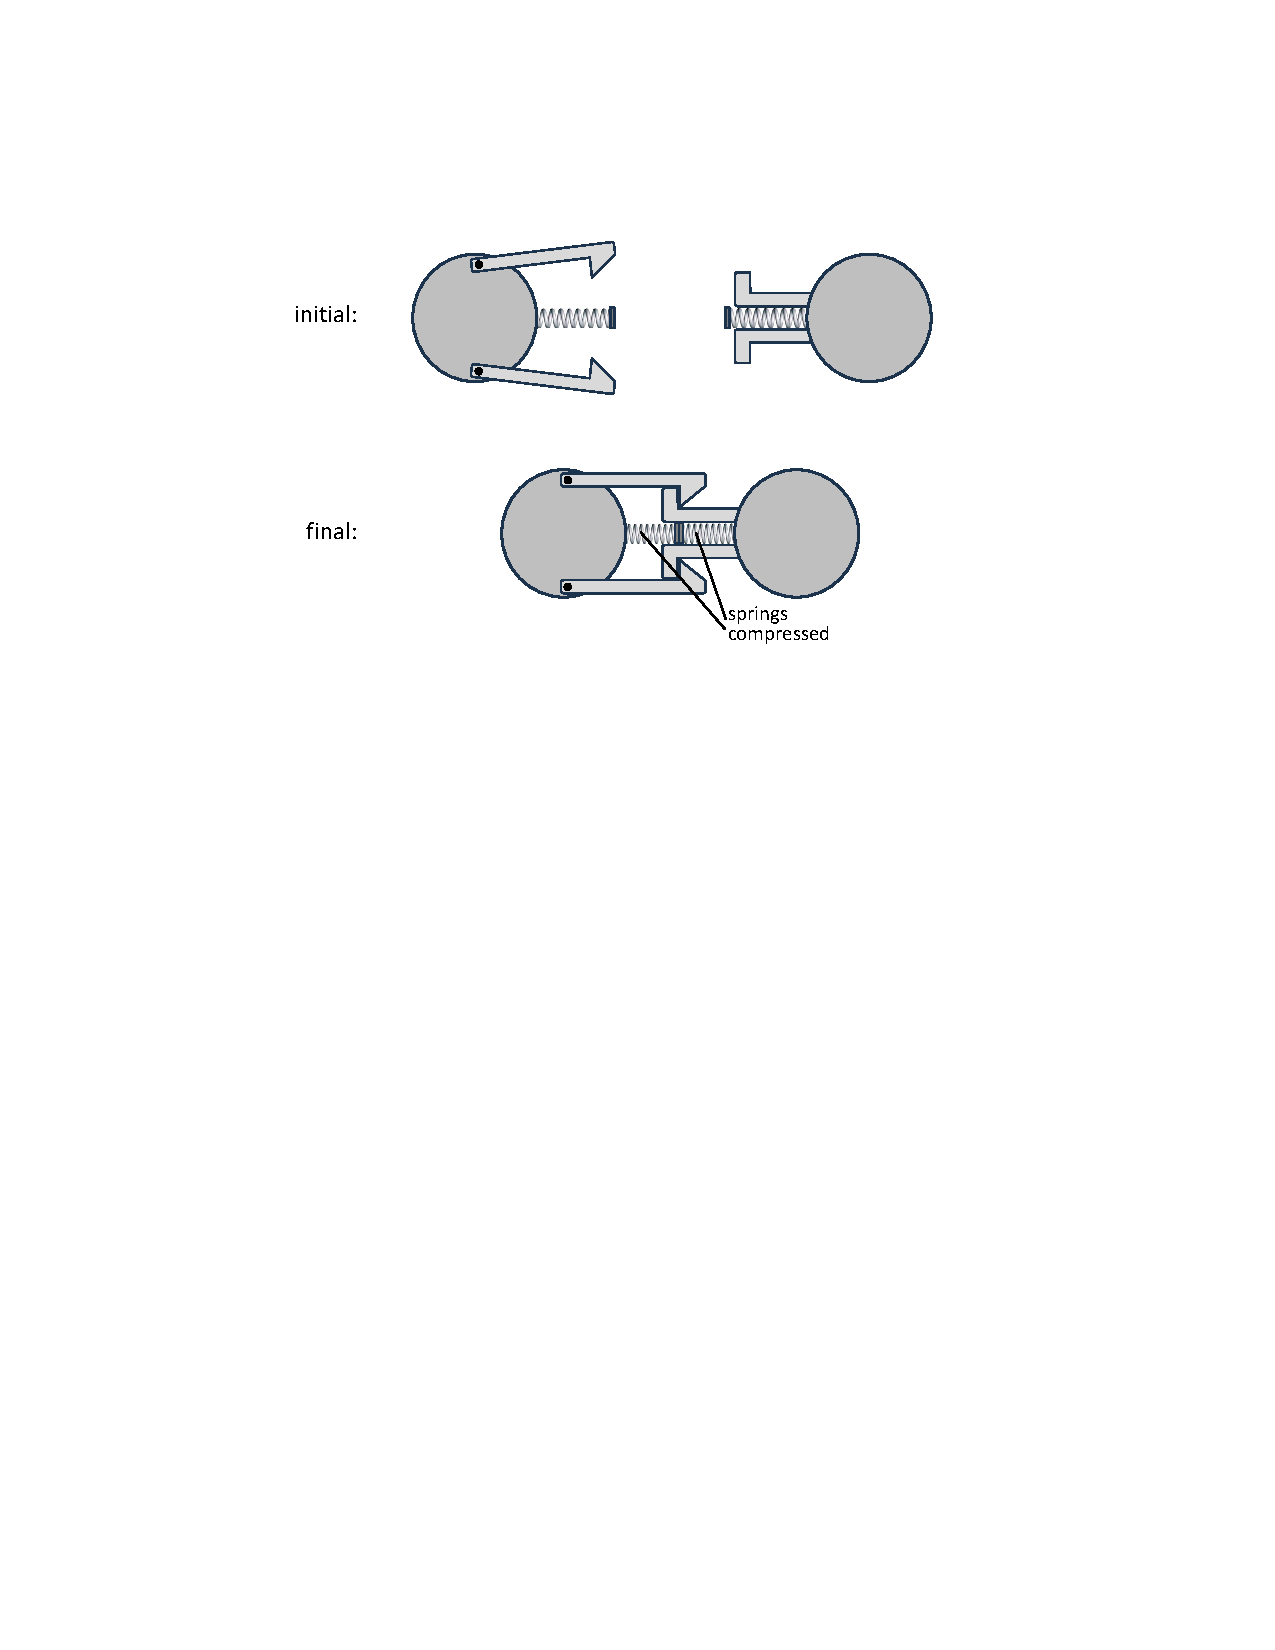
\includegraphics{energy_mass/latching.pdf}
\caption{A latching mechanism that makes the particles stick together.}
\end{center}
\end{figure}


\begin{enumerate}[labparts]

\item Suppose that in Bob's reference frame, there is \textit{just barely} enough kinetic energy converted to compressing the springs that the latch closes, and the particles remain together.  Do the particles also remain together after the collision in Anna's reference frame?
\answerspace{0.2in}

\item Suppose that in Bob's reference frame, there is \textit{not quite} enough kinetic energy converted to compressing the springs to allow the latch to close, and the particles fly apart after the collision.  Do the particles also fly apart after the collision in Anna's reference frame?
\answerspace{0.2in}

\item Do Anna and Bob always agree about whether the particles remain together or fly apart after the collision, bearing in mind that the correct answer is ``yes''?
\answerspace{0.2in}

\item Do Anna and Bob agree about how much energy goes into compressing the springs?
\answerspace{0.2in}

\item Thus, do Anna and Bob agree on the change in kinetic energy $\Delta K$ during the collision, again bearing in mind that the correct answer is ``yes''?
\label{part_Anna_and_Bob_must_agree}
\answerspace{0.2in}

Great!  Now all you need to do is verify that Anna's value of $\Delta K$ matches Bob's in the figure below!

\begin{figure}[h!]
\begin{center}
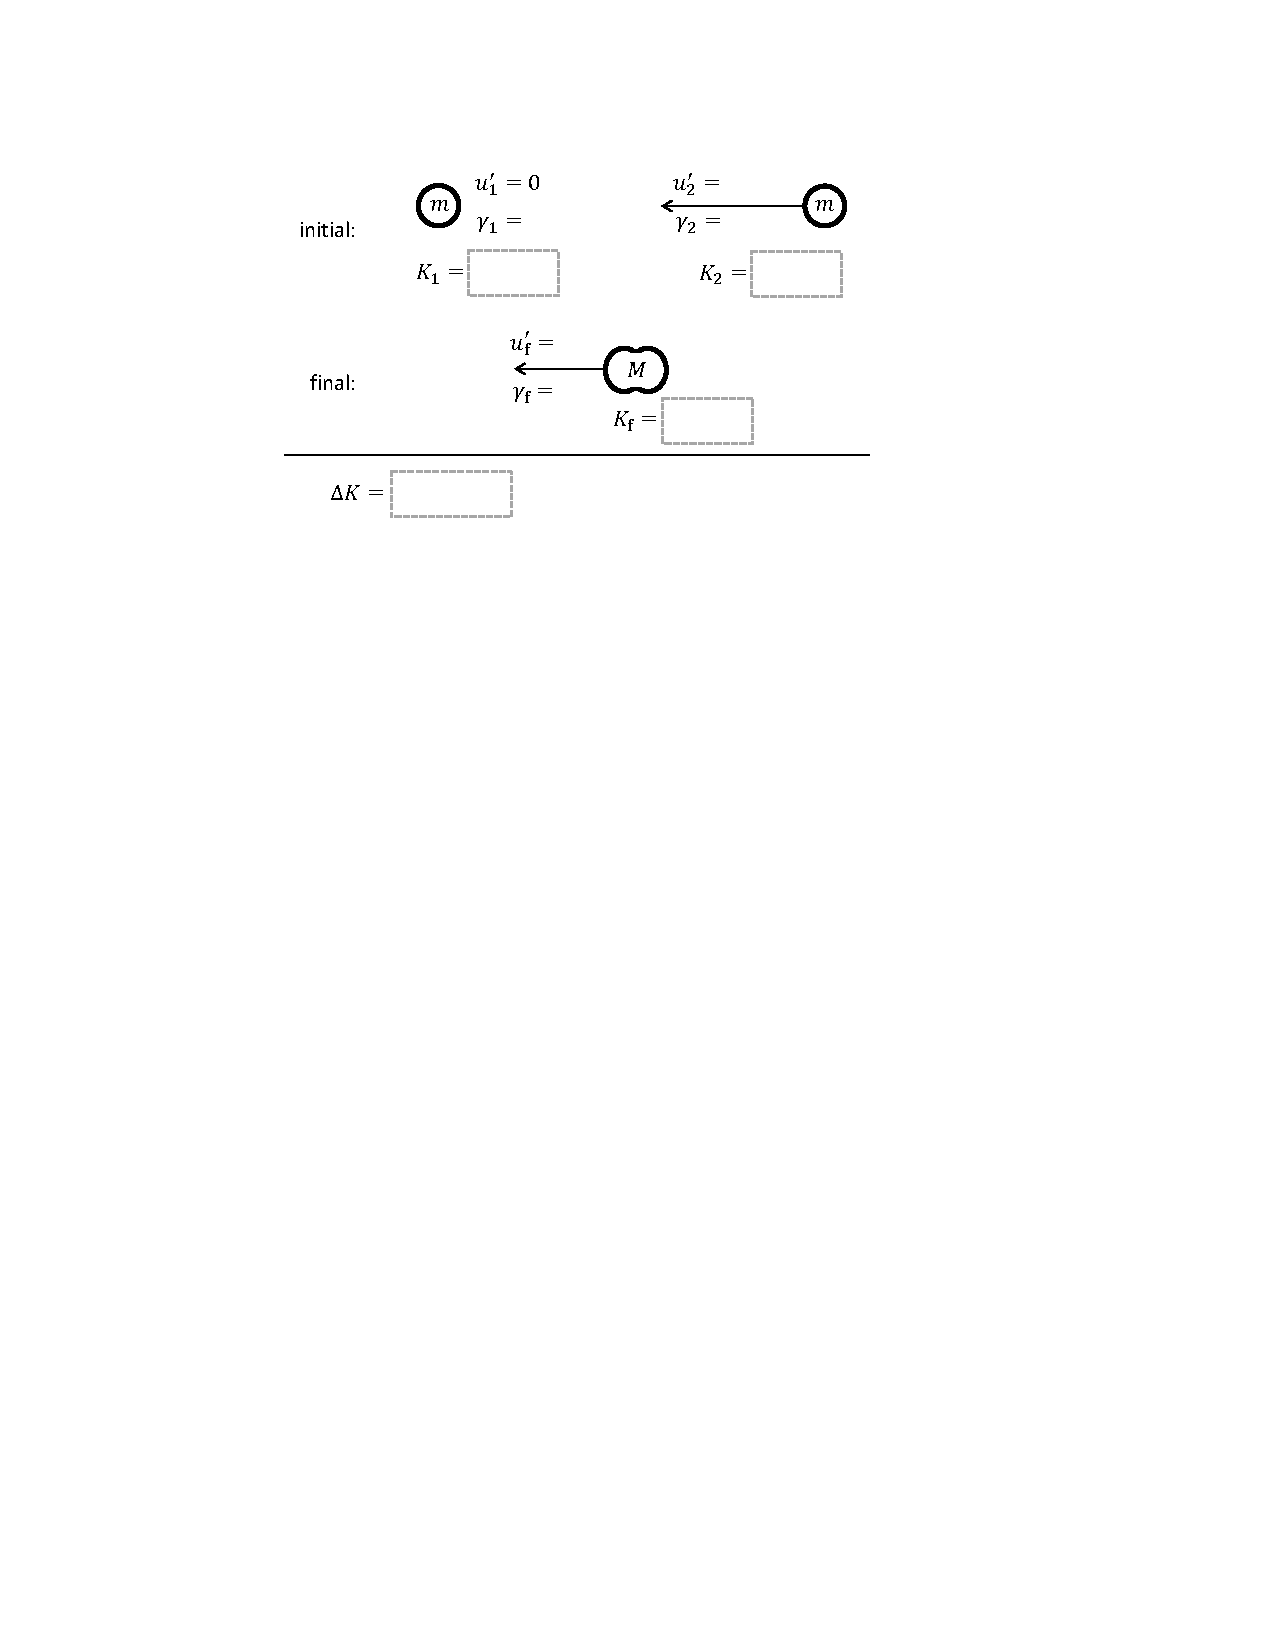
\includegraphics{energy_mass/collision_m_and_m_anna_with_k.pdf}
\caption{Anna's reference frame again, this time with $\gamma$ and $K$.}
\end{center}
\end{figure}

\item Copy the speeds $u'$ from Figure~\ref{figure_collision_m_and_m_anna_no_k}, and calculate the values of $\gamma$ and $K$ for each particle.  
\answerspace{0.8in}

\item Does your value of $\Delta K$ for Anna agree with your value of $\Delta K$ for Bob?
\answerspace{0.2in}

\end{enumerate}
\pagebreak

\textbf{What Went Wrong?}

Well, shoot.  Anna's value of $\Delta K$ didn't agree with Bob's value of $\Delta K$.  Yet we said in Part~\ref{part_Anna_and_Bob_must_agree} of Activity~2 that they \textit{have to} agree.  So what went wrong?

What went wrong is that you probably assumed that mass was conserved, along with energy---just as it was in Activity~2 of Lab~\ref{lab_energy_mass_warmup}, when a shell exploded into two fragments.  Similarly, you naturally assumed here that the total mass of the resulting particle after the collision was $M=2m$.  And you were wrong. :-)

In fact, Einstein found\footnote{In yet another paper published in 1905---again, having a good year!} that mass and energy are interchangeable.  Or, put another way, that mass is just another form of energy.  Energy and mass are still conserved, but they are conserved \textit{collectively, together}.  The true total energy of a particle $E_{\rm total}$ actually consists of two parts,
\begin{equation}
E_{\rm total}=K+E_{\rm internal},
\label{eq:E_total}
\end{equation}
where $K$ is still the kinetic energy, and the internal energy $E_{\rm internal}$ of a particle is defined by the most famous physics equation in the world,
\begin{equation}
E_{\rm internal} = mc^2.
\end{equation}
Combining Equations~\ref{eq:K_relativistic} and~\ref{eq:E_total}, we can also write $E_{\rm total}$ as
\begin{alignat}{3}
%\begin{split}
E_{\rm total} &=\qquad K & +  \quad & E_{\rm internal} \nonumber \\
& =  (\gamma-1)mc^2 \quad & + \quad & mc^2 \nonumber \\
& = ~ \gamma mc^2.
%\end{split}
\end{alignat}


\textbf{Activity 3: Getting Conservation of Energy Right}

In this part, we'll redo the parts of the previous activities that we didn't get right, applying Equation~\ref{eq:E_total} to the collision.

\begin{enumerate}[labparts]

\item Verify that your values in Figure~\ref{figure_collision_m_and_m_bob} on page~\pageref{figure_collision_m_and_m_bob} are correct: $K_1=K_2=0.25mc^2$, $K_{\rm f}=0$, and $\Delta K = -0.5mc^2$.  These should all be okay, because even though you may have imagined that $M=2m$ (wrong), it didn't affect your values because the mass $M$ particle wasn't moving anyway.


\item Mark the parts of the Activity~2 that you got wrong.  Put a giant ``{\Large {$\times$}}'' over the boxes for $K_{\rm f}$ and $\Delta K$ in Figure~4 (perhaps with a note like ``Wrong---see Activity 3''), and make any additional notes in the margins of parts (f) and (g) that you wish.


\item In Figure~5 on the following page, calculate $K_1$ and $K_2$, verifying that they are the same as you calculated in Figure~4. 
\answerspace{0.6in}

\begin{figure}[t]
\begin{center}
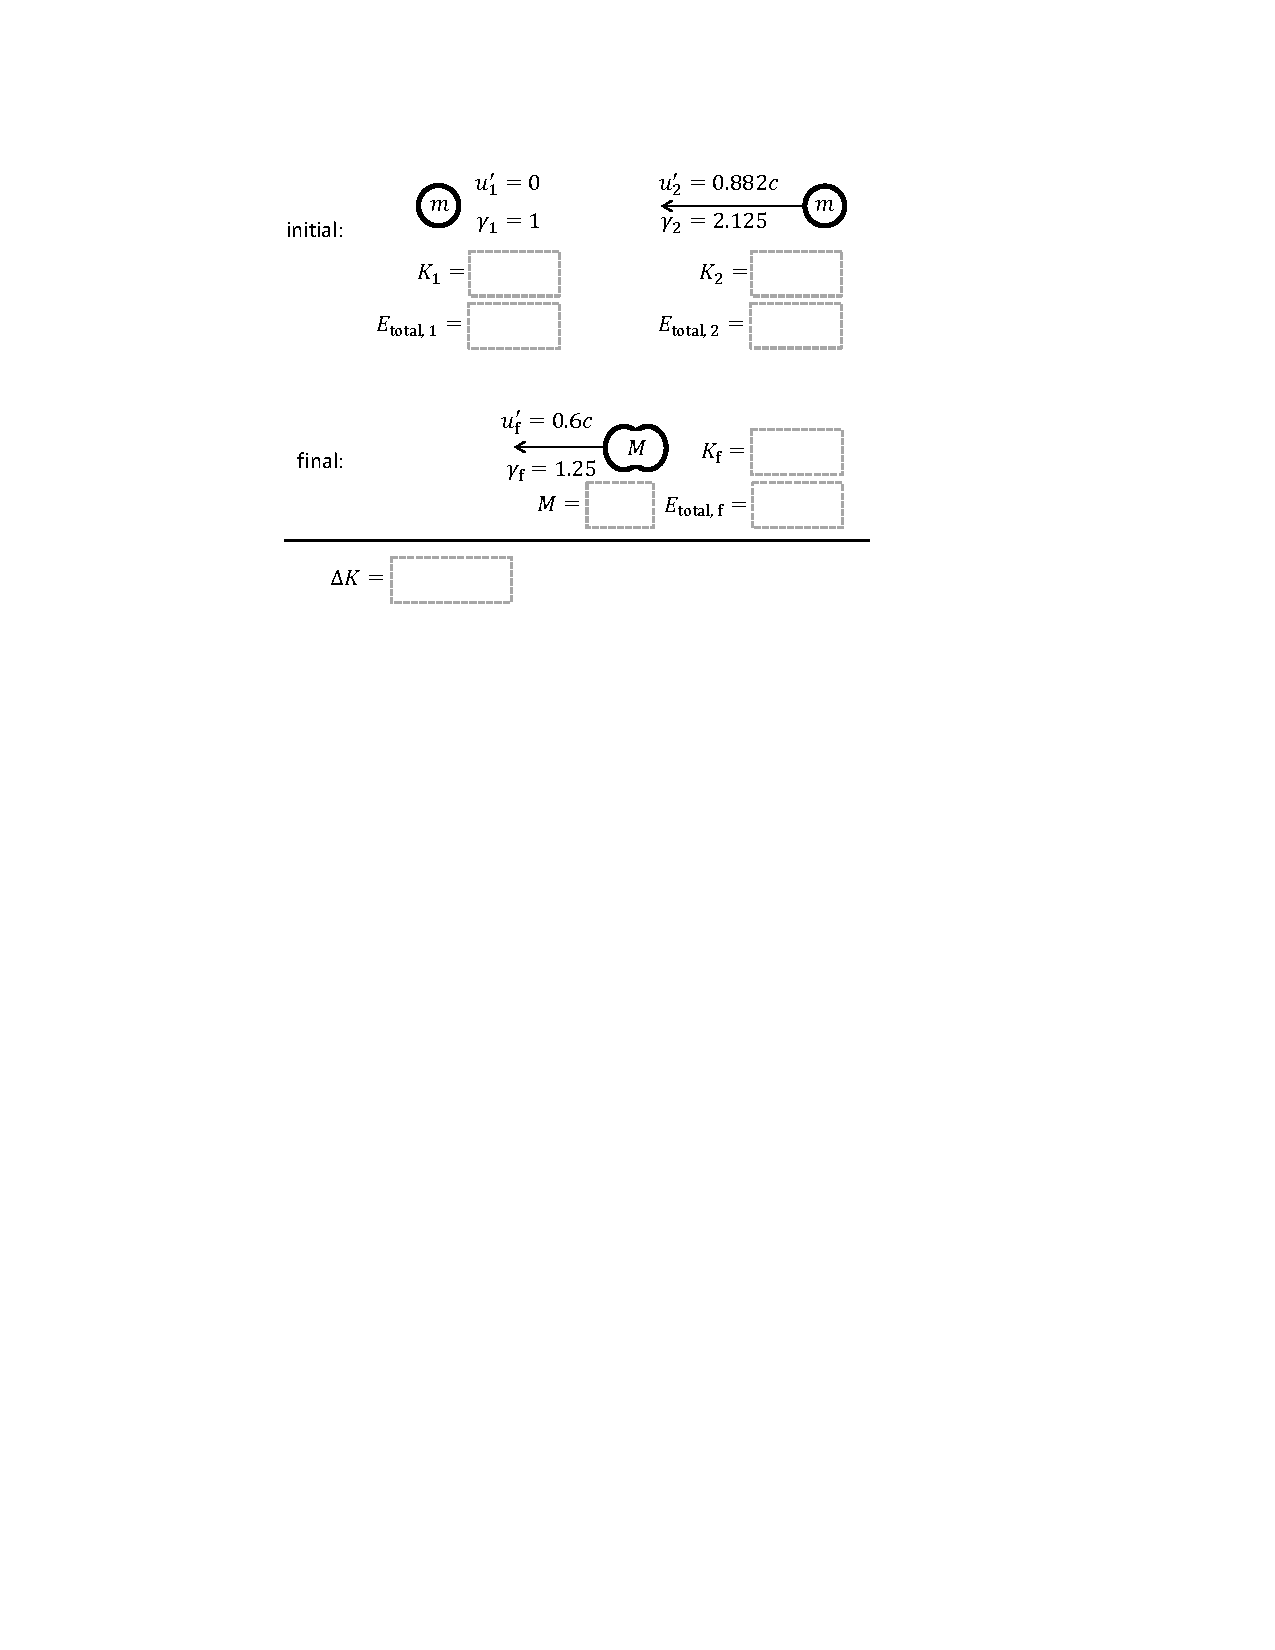
\includegraphics{energy_mass/collision_m_and_m_anna_final.pdf}
\caption{Anna's reference frame again.  This time we'll get it right for sure!}
\end{center}
\end{figure}


\item In Figure~5, calculate the total energies $E_{\rm total,1}$ and $E_{\rm total,2}$ of the two initial particles.
\answerspace{0.6in}

\item From your previous answer, what is the total energy $E_{\rm total,f}$ of the final particle, in terms of $m$?  (Hint: the total energy must be conserved.)
\answerspace{0.4in}

\item The total energy of final particle can also be expressed as $E_{\rm total,f} = \gamma Mc^2$.  What is the mass $M$ of the final particle, in terms of $m$?
\answerspace{0.6in}

\item What is the kinetic energy $K_f$ of the final particle, in terms of $m$?
\answerspace{0.6in}

\item Finally, what is $\Delta K$ in this reference frame.  Does this agree with what you found in Bob's reference frame in Activity 1?
\answerspace{0.6in}
\end{enumerate}







